\section{Counting Sort}

\subsection{Introduction}
\textbf{History:}
Counting Sort was developed by Harold H. Seward in the early 1950s, often cited around 1954. It is recognized for its ability to sort integers in linear time under the right conditions.

\begin{figure}[H]
\centering
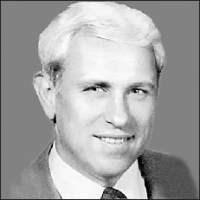
\includegraphics[scale=1]{img/haroldHSeward.jpg}
\caption{Harold H. Seward (1930-2012)}
\label{fig:harold_h_seward}
\end{figure}

\textbf{Definition:}
Counting Sort is a non-comparison-based sorting algorithm that sorts elements by counting the number of occurrences of each unique value in the input array. It then uses these counts to determine the positions of each element in the final, sorted array.

\begin{itemize}
    \item The algorithm operates in linear time.
    \item Time complexity: \(O(n + k)\), where \(n\) is the number of elements and \(k\) is the range of the input values.
\end{itemize}

\subsection{Algorithm and Implementation}
\begin{enumerate}
    \item \textbf{Determine the Range of the Data:} Sometimes min is assumed to be 0 to simplify the process.
    \item \textbf{Initialize the Count Array:} Create a count array of size \((\text{max} - \text{min} + 1)\) and initialize all elements to 0.
    \item \textbf{Count the Occurrences:} Iterate over the input array and for each element, increment the corresponding index in the count array. For an element \(x\), increment \(\text{count}[x - \text{min}]\).
    \item \textbf{Transform the Count Array into a Cumulative Count Array:} Modify the count array such that each element at index \(i\) contains the sum of previous counts. This cumulative count tells you the final position of each element in the output array.
    \item \textbf{Build the Output Array:}
    \begin{itemize}
        \item Traverse the input array once more, usually in reverse order to ensure stability (maintaining the original order of equal elements).
        \item Place each element \(x\) into its correct position in the output array by using the cumulative count, then decrement the count value for \(x\).
    \end{itemize}
\end{enumerate}

\begin{algorithm}
\caption{Counting Sort}
\begin{algorithmic}[1]
    \State \textbf{Input:} Array $A$ of size $n$
    \State \textbf{Output:} Sorted array $B$
    \Function{CountingSort}{$A$, $n$}
        \State $min \gets \min(A)$
        \State $max \gets \max(A)$
        \State $count \gets \text{array of size } (max - min + 1) \text{ initialized to 0}$
        \For{each element $x$ in $A$}
            \State $count[x - min] \gets count[x - min] + 1$
        \EndFor
        \For{$i \gets 1$ to $length(count) - 1$}
            \State $count[i] \gets count[i] + count[i - 1]$
        \EndFor
        \State $B \gets \text{array of size } n$
        \For{$i \gets 0$ to $n - 1$}
            \State $x \gets A[i]$
            \State $B[count[x - min] - 1] \gets x$
            \State $count[x - min] \gets count[x - min] - 1$
        \EndFor
        \State \textbf{Return} $B$
    \EndFunction
\end{algorithmic}
\end{algorithm}

\begin{minipage}{\linewidth}
    Below is the implementation in C++:
        \lstinputlisting[language=C++, caption=Counting Sort in C++, style=mystyle,]{code/countingSort.cpp}
\end{minipage}

\subsection{Evaluation}
\subsubsection{Building the Count Array}
\textbf{Operation:} Create and populate the count array with the frequency of each element in the input array. \\
\textbf{Complexity:} \(O(n)\) \\
\textbf{Explanation:} Each element in the input array is processed once to record its frequency in the count array.

\subsubsection{Modifying the Count Array}
\textbf{Operation:} Convert the count array into a cumulative count array, indicating the position of each element in the sorted order. \\
\textbf{Complexity:} \(O(\text{max} - \text{min} + 1)\) \\
\textbf{Explanation:} For each value in the count array, we compute a running total (cumulative sum), which takes linear time with respect to the range of values.

\subsubsection{Reconstructing the Sorted Array}
\textbf{Operation:} Use the count array to place each element from the input array into its correct position in the output array, preserving their order (stability). \\
\textbf{Complexity:} \(O(n)\) \\
\textbf{Explanation:} Each element from the input array is placed in the output array based on its position derived from the cumulative count.

\subsubsection{Space Complexity Evaluation}
\textbf{Space Used:} \(O(\text{max} - \text{min} + 1)\) \\
\textbf{Explanation:} Additional space is needed to store the count array. Its size depends on the range of values in the input array (\(\text{max} - \text{min} + 1\)).

\subsection{Application}
Counting sort is a non-comparison-based sorting algorithm that works well for sorting integers or objects with small, discrete key ranges. It counts the occurrences of each element and uses this information to place elements in their correct sorted position.
\begin{enumerate}
    \item \textbf{Sorting Small Range Integers:} Counting sort is highly efficient for sorting integers or keys within a small, known range. \textit{Example:} Sorting exam scores (e.g., 0 to 100) or ages of individuals.
    \item \textbf{Histogram Generation:} Counting sort can be used to generate histograms or frequency distributions of data. \textit{Example:} Analyzing the frequency of words in a text or the distribution of pixel intensities in an image.
    \item \textbf{Data Compression:} Counting sort is used in data compression algorithms to analyze and organize data frequencies. \textit{Example:} Building frequency tables for Huffman coding or other compression techniques.
    \item \textbf{Counting Occurrences:} Counting sort can be used to count the occurrences of elements in a dataset. \textit{Example:} Counting the number of students who scored a particular grade in an exam.
    \item \textbf{Sorting Characters or Small Alphabets:} Counting sort is efficient for sorting characters or small alphabets. \textit{Example:} Sorting letters in a word or DNA sequences (A, T, C, G).
    \item \textbf{Real-Time Systems:} Counting sort is used in real-time systems where sorting needs to be done quickly and efficiently. \textit{Example:} Sorting sensor data in real-time for IoT devices.
    \item \textbf{Database Indexing:} Counting sort can be used in database systems to sort and index records with small key ranges. \textit{Example:} Sorting records by a small set of categories or flags.
    \item \textbf{Statistical Analysis:} Counting sort is used in statistical analysis to sort and analyze data distributions. \textit{Example:} Sorting survey responses or experimental data for further analysis.
    \item \textbf{String Sorting:} Counting sort is used in string sorting algorithms, especially when sorting by a specific character position. \textit{Example:} Sorting strings lexicographically or by a specific attribute.
\end{enumerate}

\subsection{Problems}

\subsubsection{Sort Colors}
\href{https://leetcode.com/problems/sort-colors/description/}{LeetCode}

\textbf{Description:} Given an array with $n$ objects colored red, white, or blue, sort them in-place so that objects of the same color are adjacent, with the colors in the order red, white, and blue.

\textbf{Detailed Instructions:}
\begin{enumerate}
    \item Initialize Pointers: Set three pointers: low, mid, and high. Initialize low and mid to the start of the array and high to the end.
    \item Iterate Through the Array:
    \begin{itemize}
        \item While mid is less than or equal to high:
        \item If array[mid] is 0, swap it with array[low], increment both low and mid.
        \item If array[mid] is 1, just increment mid.
        \item If array[mid] is 2, swap it with array[high] and decrement high.
    \end{itemize}
    \item Complete the Sorting: Continue until mid exceeds high.
    \item Return the Sorted Array.
\end{enumerate}

\subsubsection{Counting Sort 1}
\href{https://www.hackerrank.com/challenges/one-week-preparation-kit-countingsort1/problem}{HackerRank}

\textbf{Description:} Count the frequency of each integer in an array.

\textbf{Detailed Instructions:}
\begin{enumerate}
    \item Identify the maximum value in the array to determine the size of your count array.
    \item Traverse the input array, incrementing the corresponding index in the count array for each element encountered.
    \item Output the count array, ensuring that the frequency for every number (including those with zero occurrences) is reported.
\end{enumerate}

\subsubsection{The Full Counting Sort}
\href{https://www.hackerrank.com/challenges/countingsort4/problem}{HackerRank}

\textbf{Description:} Sort pairs of numbers and strings based on numeric keys while preserving the original order for equal keys.

\textbf{Detailed Instructions:}
\begin{enumerate}
    \item Create a count array based on the numeric keys and count the occurrences.
    \item Convert the count array into a cumulative frequency array to determine the final positions of the keys.
    \item Place each (number, string) pair into a new array at the position determined by the cumulative counts, ensuring that elements with the same key retain their original order (stability).
\end{enumerate}

\subsubsection{Counting Sort 2}
\href{https://www.hackerrank.com/challenges/countingsort2/problem}{HackerRank}

\textbf{Description:} Efficiently sort an array of integers using counting sort.

\textbf{Detailed Instructions:}
\begin{enumerate}
    \item Find the maximum integer in the input array to allocate a count array of size \(\text{max}+1\).
    \item Iterate through the array to populate the count array with frequencies of each integer.
    \item Reconstruct the sorted array by iterating through the count array and appending each integer based on its count, ensuring linear time performance when the range isn’t excessively large.
\end{enumerate}

\subsubsection{Find All Numbers Disappeared in an Array}
\href{https://leetcode.com/problems/find-all-numbers-disappeared-in-an-array/}{LeetCode}

\textbf{Description:} Identify which numbers in the range [1, n] are missing from the input array.

\textbf{Detailed Instructions:}
\begin{enumerate}
    \item Create a boolean (or count) array of size \(n+1\), initialized to mark all numbers as missing.
    \item Traverse the input array and mark each number that appears in the corresponding index of your boolean array.
    \item Iterate through the range 1 to \(n\) and collect those numbers that remain unmarked, as these are the missing numbers. This counting technique ensures that every potential number is checked exactly once.
\end{enumerate}